\chapter{Experiment and Result}
\section{Teori}
\subsection{Klasifikasi Teks}
\subsubsection{Pengertian Klasifikasi Teks}
Merupakan salah satu tugas terpenting dalam Pemrosesan Bahasa Alami (Natural Language Processing). Ini adalah proses mengklasifikasikan string teks atau dokumen ke dalam kategori yang berbeda, tergantung pada konten string. Klasifikasi teks memiliki berbagai aplikasi, seperti mendeteksi sentimen pengguna dari tweet, mengklasifikasikan email sebagai spam atau ham, mengklasifikasikan posting blog ke dalam kategori yang berbeda, penandaan otomatis permintaan pelanggan, dan sebagainya. BErikut adalah contoh dari Klasifikasi Teks.
Contohnya, misal kita ingin mencari kata dog, table, on, the . kemudian jika kata yang dimaksud sesuai maka akan menampilkan bilangan biner 1 dan jika salah 0. Seperti dibawah ini :
\begin{figure}[ht]
\centering
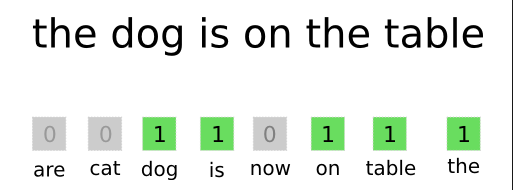
\includegraphics[scale=0.5]{figures/chapter4tasya1.png}
\caption{Klasifikasi Teks Tasya}
\label{Contoh}
\end{figure}

\subsection{Klasifikasi Bunga}
Jelaskan mengapa klasifikasi bunga tidak bisa menggunakan machine learning, sertakan ilustrasi sendiri.
Dikarenakan tidak semua bunga memliki ciri - ciri yang sama. Atau dalam kata lain terdapat data noise dalam klasifikasi bunga sehingga tidak bisa menggunakan machine learning.
Contohnya Anggrek memiliki warna ungu, dengan jumlah kelopak 5. Kemudian ada bunga warna ungu dengan jumlah kelopak yang sama namun ternyata bukan anggrek dan kategorinya banyak sekali. Bahkan ada bunga yang tidak jelas apakah warnanya sesuai atau tidak, sehingga bisa menyebabkan data noise.
\begin{figure}[ht]
\centering
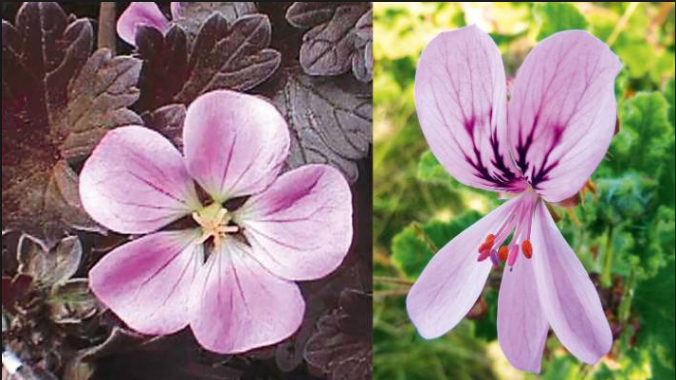
\includegraphics[scale=0.5]{figures/chapter4tasya2.png}
\caption{Klasifikasi Bunga Berwana Ungu Tasya}
\label{Contoh}
\end{figure}

\subsection{Pembelajaran Mesin Pada Teks Kata - Kata di Youtube}
Menggunakan teknik bag-of-words pada klasifikasi berbasis text dan kata untuk mengklasifikasikan komentar yang ada di internet sebagai spam atau bukan. Misalkan pada kolom komentar dapat di cek seberapa sering suatu kata muncul dalam kalimat. Setiap kata dapat dijadikan baris dan kolomnya ini merupakan kategori kata terbut, apakah masuk kedalam spam atau tidak. dan contoh lainnya yaitu pada Caption. dimana akan muncul subtitle secara otomatis dari youtube menggunakan sensor suara yang disesuaikan dengan kata yang telah ditentukan. Contohnya seperti berikut :
\begin{figure}[ht]
\centering
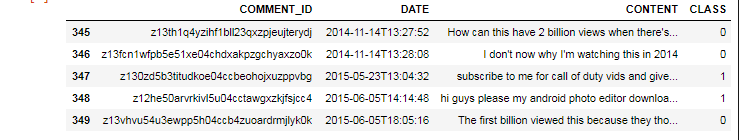
\includegraphics[scale=0.5]{figures/chapter4tasya3.png}
\caption{Klasifikasi Comment Spam Di Youtube Tasya}
\label{Contoh}
\end{figure}

\subsection{Arti Score 44\% Pada Random Forest, 27\% Pada Decission Tree Dan 29\% Dari SVM}
Itu merupakan presentase keakurasian prediksi yang dilakukan pada saat testing menggunakan label pada dataset yang digunakan. Score merupakan mendefinisikan aturan evaluasi model. Maka pada saat dijalankan akan muncuk persentase tersebut yang menunjukan keakurasian atau keberhasilan dari prediksi yang dilakukan. Jika menggunakan Random Forest maka hasilnya 40\% , jika menggunakan Decission Tree hasil prediksinya yaitu 27\% dan pada SVM 29\% .

\subsection{Bag of Words}
\subsubsection{Pengertian Bag of Words}
Merupakan representasi teks yang menggambarkan kemunculan kata-kata dalam dokumen. ePngelompokan kata kata kedalam perhitunga, berapakali sebuah kata muncul dalam satu kalimat. Disebut "tas" kata-kata, karena informasi tentang susunan atau struktur kata dalam dokumen dibuang. Model ini hanya berkaitan dengan apakah kata-kata yang diketahui muncul dalam dokumen, bukan di mana dalam dokumen.\\
Contohnya disini akan melihat kemunculan kata dari kalimat :
\begin{enumerate}
\item I Love Dogs
\item I hate dogs and knitting
\item Knitting is my hobby and passion.
\end{enumerate}
\begin{figure}[ht]
\centering
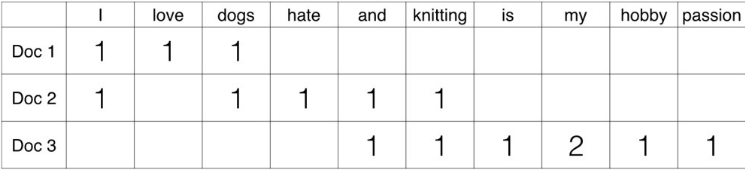
\includegraphics[scale=0.5]{figures/chapter4tasya4.png}
\caption{Bag of Words Tasya}
\label{Contoh}
\end{figure}

\subsection{TF-IDF}
TF-IDF  memberi kita frekuensi kata dalam setiap dokumen dalam korpus atau mengganti data jadi number. Ini adalah rasio berapa kali kata itu muncul dalam dokumen dibandingkan dengan jumlah total kata dalam dokumen itu. Itu meningkat seiring jumlah kemunculan kata itu di dalam dokumen meningkat. Setiap dokumen memiliki tf sendiri. Dalam ilustrasi disini saya akan mengganti contoh Bag of Words menjadi bentuk TF-IDF.
\begin{figure}[ht]
\centering
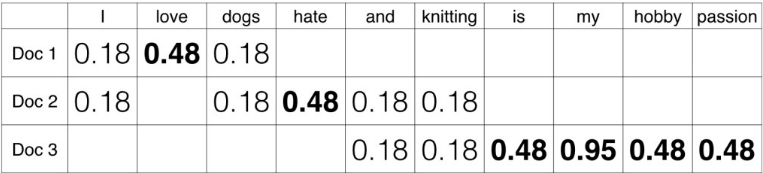
\includegraphics[scale=0.5]{figures/chapter4tasya5.png}
\caption{Contoh TF-IDF Tasya}
\label{Contoh}
\end{figure}

\section{PRAKTIKUM}
\subsection{Aplikasi Sederhana Menggunakan Pandas}
Disini saya akan menggunakana Dataset dari https://www.kaggle.com/spscientist/students-performance-in-exams dan akan mengambil Data Dummy sebanyak 500 records dan membuat Dataframe baru.
\begin{verbatim}
import pandas as pd
mhs = pd.read_csv('StudentsPerformanceExam.csv', sep=';')
df = pd.DataFrame(mhs, columns = ['gender', 'race/ethnicity', 'parental level of education', 'lunch', 'test preparation course', 'math score', 'reading score', 'writing score'])

dummy = pd.get_dummies (df['test preparation course'])
dummy.head()

df = df.join(dummy)
\end{verbatim}
Maksud dari kodingan diatas yaitu :
\begin{enumerate}
\item Baris pertama impor librari pandas dengan inisiasi pd
\item Definisikan variabel mhs untuk membaca file csv dengan pandas
\item variabel df akan menggunakan function pddataframe untuk membuat datafarme di pandas dari file CSV yang tadi.
\item Mendefinisikan variabel dummy untuk mengubah data categorical menjadi integer. dibahwa merupakan data sebelum di Dummy.
\begin{figure}[ht]
\centering
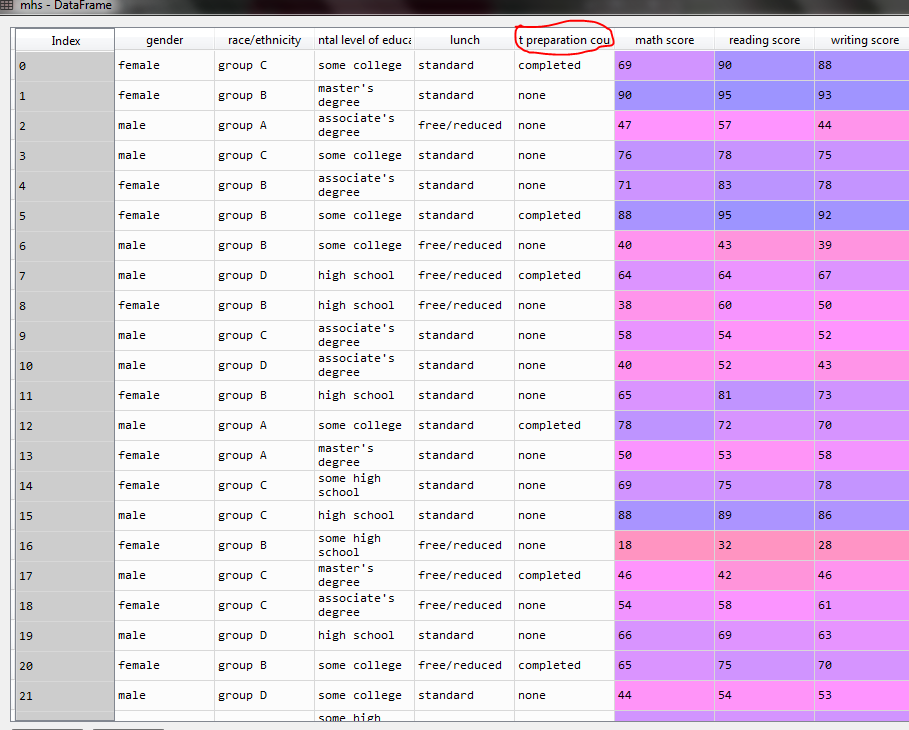
\includegraphics[scale=0.5]{figures/praktektasya2.png}
\caption{Dataset Original Tasya}
\label{Aplikasi Pandas}
\end{figure}

\item Atribut atau kolom yang ingin di Dummy yaitu test preparation course. Dalam test preparation course terdapat dua value yaitu Completed dan none. Yang jika di dummy maka valuenya akan berubah menjadi 1 dan 0 seperti berikut :
\begin{figure}[ht]
\centering
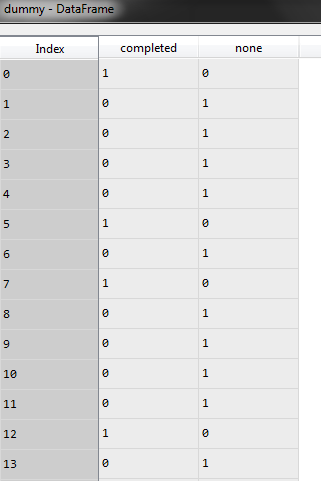
\includegraphics[scale=0.5]{figures/praktektasya3.png}
\caption{Dataset Dummy Tasya}
\label{Aplikasi Pandas}
\end{figure}
\item kemudian df akan melakukan join dengan dataframe dummy.
\end{enumerate}

\subsection{Memecah DataFrame Menjadi 2 Dataframe}
Dari dataframe tersebut dipecah menjadi dua dataframe yaitu 450 row pertama dan 50 row sisanya
\begin{verbatim}
mhs_train= mhs[:450]
mhs_test= mhs[451:]
\end{verbatim}
\begin{enumerate}
\item mhs train akan mendefinisikan dataframe untuk train dengan 450 data pertama
\item mhs test mendefinisikan dataframe untuk test untuk data setelah 451. Hasilnya seperti berikut :
\end{enumerate}
\begin{figure}[ht]
\centering
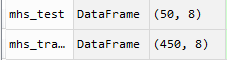
\includegraphics[scale=0.5]{figures/praktektasya4.png}
\caption{Split DataFrame Tasya}
\label{Aplikasi Pandas}
\end{figure}

\subsection{ Vektorisasi Dan Klasifikasi Dari Data Youtube Eminem Dengan Decision Tree}
\begin{enumerate}
\item Ini hasil dari impor dataset
\begin{figure}[ht]
\centering
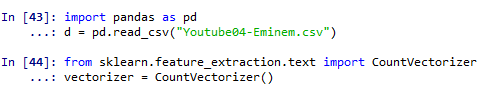
\includegraphics[scale=0.5]{figures/praktektasya7.png}
\caption{Dataset Youtube Eminem Tasya}
\label{Praktek}
\end{figure}
\item Ini hasil Setelah di Klasifikasikan dengan Decision Tree
\begin{figure}[ht]
\centering
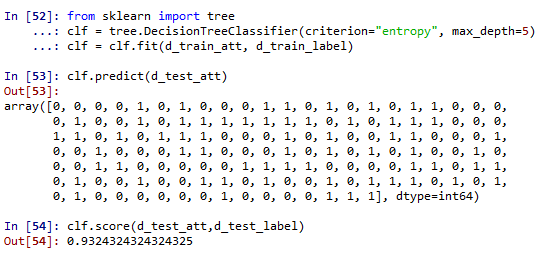
\includegraphics[scale=0.5]{figures/praktektasya6.png}
\caption{Dataset Youtube Eminem Tasya}
\label{Praktek}
\end{figure}
\item Dalam in 52 impor Tree dari Sklearn. Dan mendefinisikan variabel clf untuk memanggil Decision Tree Classifier dan melakukan fit atau pengujian
\item Dalam In 53 menggunakan prediksi untuk clf dengan function predict  untuk memprediksi test. Dan hasilnya muncul dalam bentuk array.
\item clf score memunculkan akurasi prediksi yang dilakukan terhadap clf.
\end{enumerate}

\subsection{Vektorisasi Dan Klasifikasi Dari Data Youtube Eminem Dengan SVM}
\begin{figure}[ht]
\centering
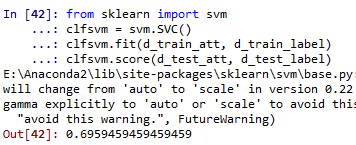
\includegraphics[scale=0.5]{figures/praktektasya8.png}
\caption{Dataset Youtube Eminem SVM Tasya}
\label{Praktek}
\end{figure}
Dari Gambar diatas dapat dijelaskan bahwa :
\begin{enumerate}
\item Impor SVM dari sklearn
\item Melakukan fit dari d train att dan d train label atau disebut dengan pengujian
\item Mendefinisikan variabel clf untuk melakukan prediksi dataset Youtube Eminem dengan SVM. Dan akan muncul hasil prediksinya
\end{enumerate}

\subsection{Vektorisasi Dan Klasifikasi Dari Data Youtube Eminem Dengan Decision Tree 2}
\begin{figure}[ht]
\centering
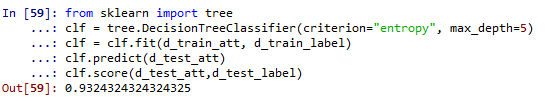
\includegraphics[scale=0.5]{figures/praktektasya9.png}
\caption{Dataset Youtube Eminem Tasya}
\label{Praktek}
\end{figure}
Maksud dari codingan diatas yaitu, mengkasifikasikan Dataset Youtube Eminem dengan Decision Tree dengan melakukan prediksi menggunakan function test pada d test att, dan memberikan akurasi prediksi menggunakan prediksi score.

\subsection{Plotting Confusion Matrix}
Berikut adalah skripl dari plotting confusion matrix dari contoh yang ada pada bagian teori
\begin{verbatim}
import matplotlib.pyplot as plt
import itertools
def plot_confusion_matrix(cm, classes,
                          normalize=False,
                          title='Confusion matrix',
                          cmap=plt.cm.Blues):
    """
    This function prints and plots the confusion matrix.
    Normalization can be applied by setting `normalize=True`.
    """
    if normalize:
        cm = cm.astype('float') / cm.sum(axis=1)[:, np.newaxis]
        print("Normalized confusion matrix")
    else:
        print('Confusion matrix, without normalization')

    print(cm)

    plt.imshow(cm, interpolation='nearest', cmap=cmap)
    plt.title(title)
    #plt.colorbar()
    tick_marks = np.arange(len(classes))
    plt.xticks(tick_marks, classes, rotation=90)
    plt.yticks(tick_marks, classes)

    fmt = '.2f' if normalize else 'd'
    thresh = cm.max() / 2.
    #for i, j in itertools.product(range(cm.shape[0]), range(cm.shape[1])):
    #    plt.text(j, i, format(cm[i, j], fmt),
    #             horizontalalignment="center",
    #             color="white" if cm[i, j] > thresh else "black")

    plt.tight_layout()
    plt.ylabel('True label')
    plt.xlabel('Predicted label')


import numpy as np
np.set_printoptions(precision=2)
plt.figure(figsize=(60,60), dpi=300)
plot_confusion_matrix(cm, classes=clf, normalize=True)
plt.show()
\end{verbatim}
Hasilnya adalah sebagai berikut :
\begin{figure}[ht]
\centering
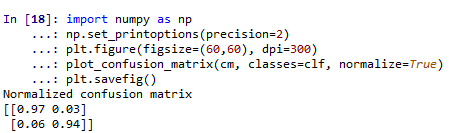
\includegraphics[scale=0.5]{figures/praktektasya10.png}
\caption{Confusion Matrix Tasya}
\label{Praktek}
\end{figure}
Dari gambar dapat dijelaskan bahwa data array merupakan data asli dan data prediksi yang dilakukan dengan Random Forest. DEngan melakukan normalisasi data confusion matrix.

\subsection{ Menjalankan Program Cross Validation}
\begin{figure}[ht]
\centering
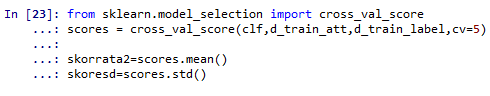
\includegraphics[scale=0.5]{figures/praktektasya5.png}
\caption{Cross Validation Tasya}
\label{Aplikasi Pandas}
\end{figure}
Gambar diatas akan dijelaskan seperti berikut :
\begin{enumerate}
\item Dari sklearn mengimpor Cross Validation
\item Variabel scores akan melakukan cross validation pada variabel clf, d train att , dan d train label
\item Variabel skorrata2 akan menghitung nilai rata rata dari variabel scores tadi menggunakan function mean
\item skoresd Menghitung standar deviasi dari data yang diberikan. Hssilnya seperti berikut :
\end{enumerate}
\begin{figure}[ht]
\centering
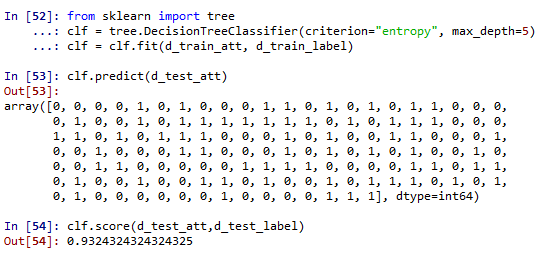
\includegraphics[scale=0.5]{figures/praktektasya6.png}
\caption{Hasil Cross Validation Tasya}
\label{Cross Validation}
\end{figure}

\subsection{Program Pengamatan Komponen Informasi}
\begin{figure}[ht]
\centering
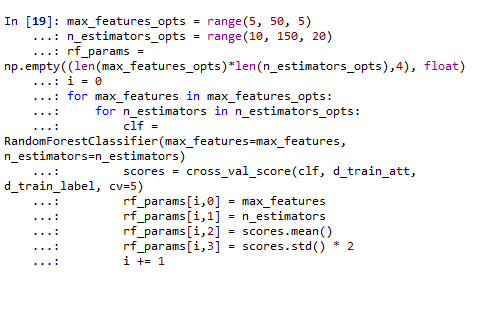
\includegraphics[scale=0.5]{figures/praktektasya11.png}
\caption{Program Komponen Informas Tasyai}
\label{Praktek}
\end{figure}
Dari gambar diatas dapat dijelaskan bahwa :
\begin{enumerate}
\item Max featuresnya dari range 5 sampai 50
\item n estimators dengan range 10 sampai 150
\item Variabel rf params berisikan function np empty dimana akan membuat array baru berisikan tipe yang didefinisikan dengan random value
\item Mendefinisika i dimulai dari angka 0 dimana max features dan n estimators menggunakan klasifikasi randomforestclassifier menggunakan data prediksi
\item Mendefinisikan rfparams untuk max features , n estimators, nilai rata dan std
\end{enumerate}

\section{Penanganan Error}
\subsection{Error Index}
\begin{enumerate}
	\item
Berikut ini merupakan eror yang didapatkan saat menjalankan program diatas
\begin{figure}[ht]
\centering
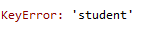
\includegraphics[scale=0.5]{figures/praktektasyaeror1.png}
\caption{Error Key Tasya }
\label{Error}
\end{figure}
\item
Pada gambar diatas kode erornya adalah KeyEror. Eror ini terjadi karena keyword yang dimasukan tidak ada.
\item
Solusi yang bisa dilakukan untuk mengatasi eror tersebut adalah sebagai berikut :
\end{enumerate}
\begin{itemize}
\item
\begin{figure}[ht]
\centering
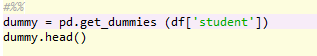
\includegraphics[scale=0.5]{figures/praktektasyaeror2.png}
\caption{Error Key Tasya}
\label{Error}
\end{figure}
Pada gambar diatas Dataset StudentPerformanceExam tidak terdapat atribut student, maka dari itu kita harus merubahnya dengan atribut yang terdapat di dataset tersebut. Mari kita gunakan atribut gender. Ubah skrip menjadi seperti berikut
\item
\begin{figure}[ht]
\centering
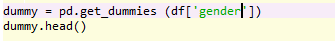
\includegraphics[scale=0.5]{figures/praktektasyaeror3.png}
\caption{Error Key Tasya}
\label{Error}
\end{figure}
\item Maka ketika di run akan muncul data dummy nya seperti berikut
\begin{figure}[ht]
\centering
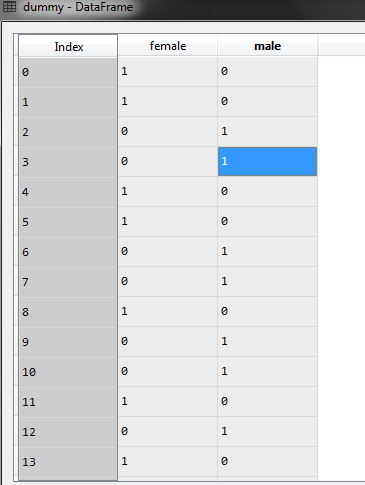
\includegraphics[scale=0.5]{figures/praktektasyaeror4.png}
\caption{Error Key Tasya}
\label{Error}
\end{figure}
\end{itemize}

